\chapter{Bedienungsanleitung}\label{bedienungsanleitung}
\section{Installation der Software}
Eclipse Installationsdialog mit Menu \textit{Hilfe / Neue Software installieren} öffnen.
 \begin{figure}[H]
  	\centering
    	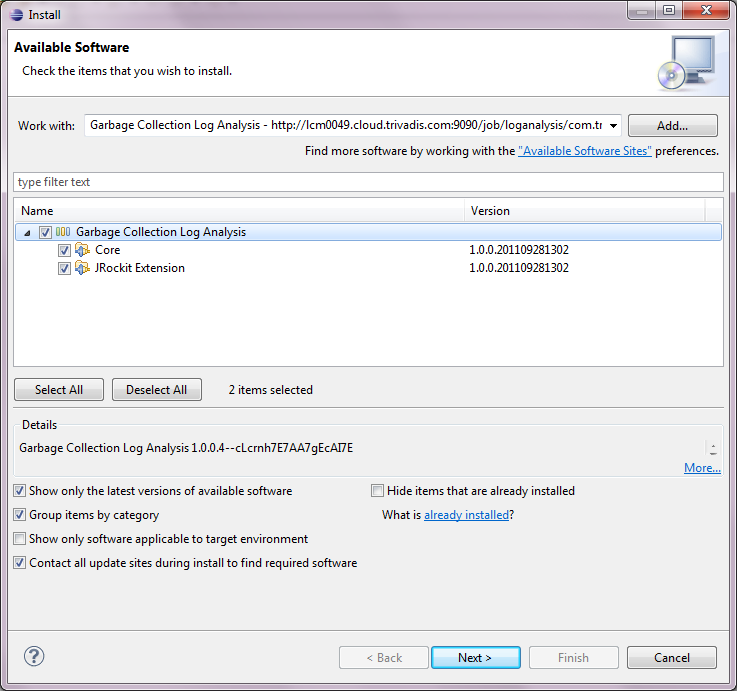
\includegraphics[width=10cm]{images/tutorial_install01}
        	\caption{Installation Garbage Collection Log Analyse}
\end{figure}
Durch Angabe der Update-Seite können danach beide Features ausgewählt werden. Nach zweimaligem Klick auf \textit{Weiter} und anschliessender Bestätigung der Lizenzbestimmungen wird die Software installiert. Danach muss die Entwicklungsumgebung neu gestartet werden.


\section{Update}
Wenn ein Update der Software verfügbar ist, kann via \textit{Hilfe / Nach Updates suchen} das Update-Fenster geöffnet werden. Die  Softwarepakete werden wenn gewünscht heruntergeladen und aktualisiert.
 \begin{figure}[H]
  	\centering
    	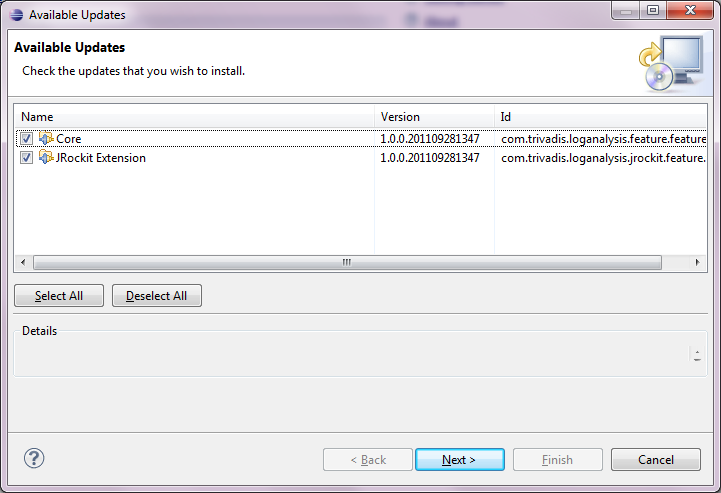
\includegraphics[width=10cm]{images/tutorial_update01}
        	\caption{Update Garbage Collection Log Analyse}
\end{figure}

\section{Dashboard}
Nach der Installation kann über den Knopf \textit{GC Log Analyse Dashboard} in der Toolbar das Dashboard geöffnet werden. 
 \begin{figure}[H]
  	\centering
    	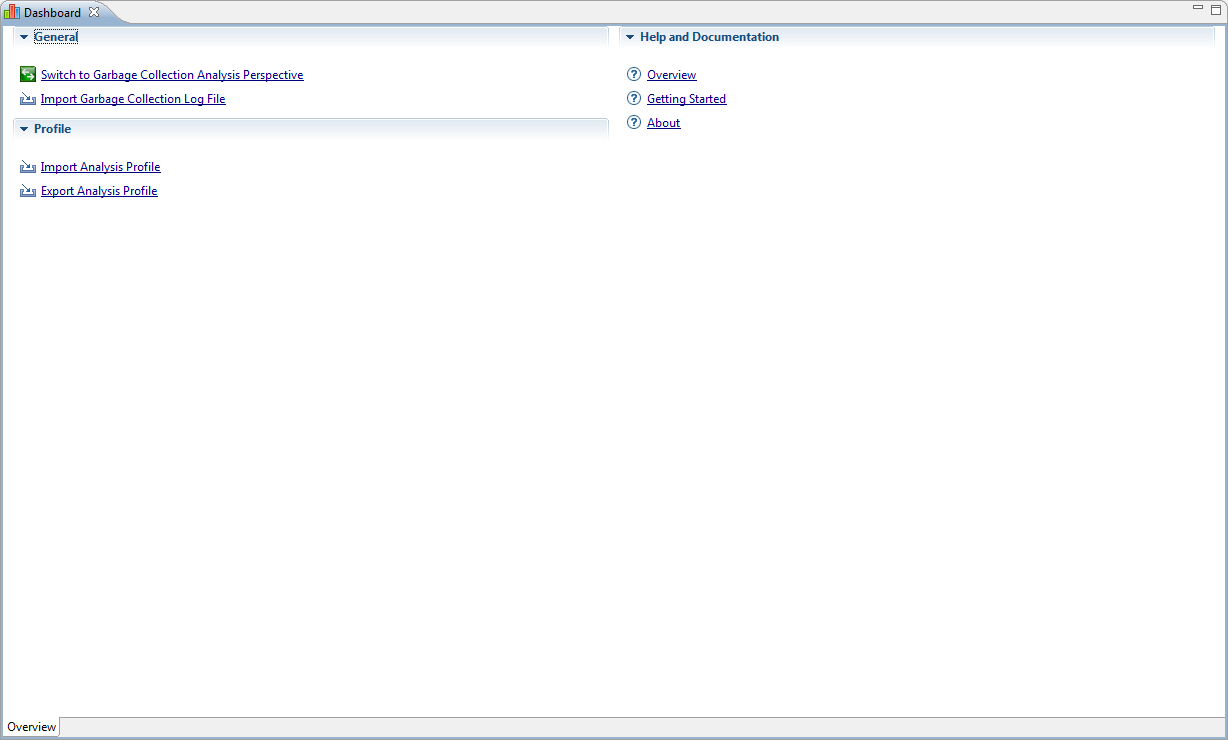
\includegraphics[width=16cm]{images/tutorial_dashboard}
        	\caption{Dashboard}
\end{figure}

Auf dem Dashboard befinden sich verschiedene Abschnitte mit unterschiedlichen Funktionen:
\begin{itemize}
	\item Generell 
		\begin{itemize}
			\item Wechsel in die Garbage Collection Perspektive
			\item Import einer Garbage Collection Logdatei
		\end{itemize}
	\item Profile
		\begin{itemize}
			\item Import eines Analyseprofils
			\item Export eines Analyseprofils
		\end{itemize}
	\item Hilfe und Dokumentation
		\begin{itemize}
			\item Beinhaltet Links auf verschiedene Inhalte der Hilfe
		\end{itemize}
\end{itemize}

\section{Import einer Garbage Collection Logdatei}
Der Import-Wizard kann auf verschiedene Arten geöffnet werden:
\begin{itemize}
	\item Über Rechtsklick auf die View \textit{Logdateien} / \textit{Import Garbage Collection Logdatei}.
	\item Über \textit{File / Import / Import Garbage Collection Logdatei} (Kategorie: Garbage Collection)
	\item Im Dashboard über \textit{Import Garbage Collection Logdatei}
\end{itemize}

Über den \textit{Browse} Button muss der Ordner angegeben werden, welcher die Logdateien beinhaltet. Anschliessend kann die Logdatei im darunterliegenden Fenster selektiert werden. Mit Klick auf \textit{Finish} wird die Datei importiert.
 \begin{figure}[H]
  	\centering
    	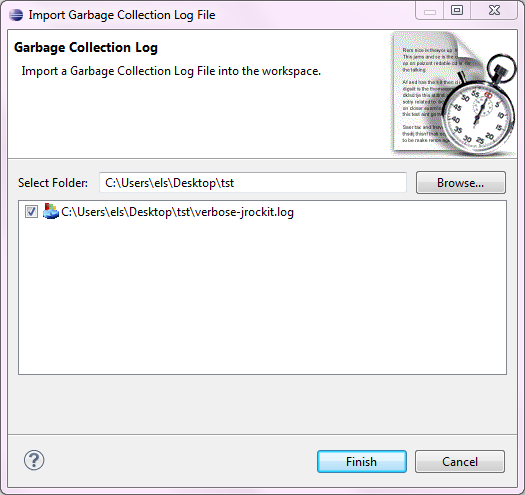
\includegraphics[width=10cm]{images/tutorial_importlog}
        	\caption{Profil importieren}
\end{figure}

\section{Profile}
Zur Verwaltung der verschiedenen Analyseprofile gibt es die View \textit{Profile}. In ihr können Profile erstellt, exportiert und importiert werden. Wenn eine Logdatei mit einem bestimmten Analyseprofil geöffnet werden soll, muss das entsprechende Profil darin selektiert sein.

\subsection{Profil erstellen}
Mit Rechtsklick auf die Ansicht \textit{Profile / Profil erstellen} oder \textit{Datei / Neu / Andere... / Analyse Profil} (Kategorie Garbage Collection) kann der Dialog zum Erstellen eines neuen Profils geöffnet werden. 
 \begin{figure}[H]
  	\centering
    	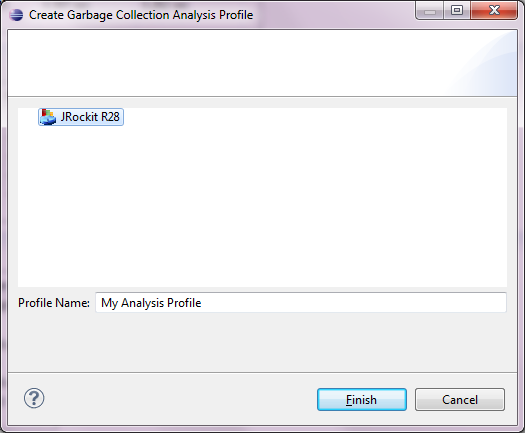
\includegraphics[width=10cm]{images/tutorial_newprofile}
        	\caption{Profil erstellen}
\end{figure}
Sofern die Erweiterung, für die das Profil erstellt wird, selektiert und ein Name vergeben ist, wird mittels Klick auf \textit{Fertigstellen} das Profil angelegt.

\subsection{Profil exportieren}
Mit Rechtsklick auf die Ansicht \textit{Profile} und Auswahl von \textit{Profil exportieren}, können die Profile in eine Lap\footnote{Lap steht für Log Analysis Profile}-Datei exportiert werden.
 \begin{figure}[H]
  	\centering
    	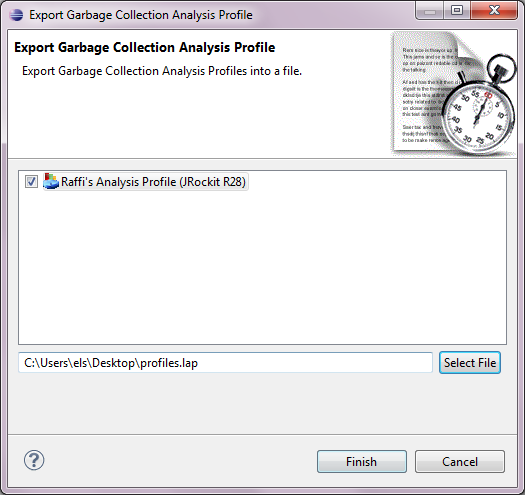
\includegraphics[width=10cm]{images/tutorial_exportprofile}
        	\caption{Profil exportieren}
\end{figure}

\subsection{Profil importieren}

Mit Rechtsklick auf die Ansicht \textit{Profile / Profil Importieren} können die Profile aus einer Lap-Datei importiert werden.
 \begin{figure}[H]
  	\centering
    	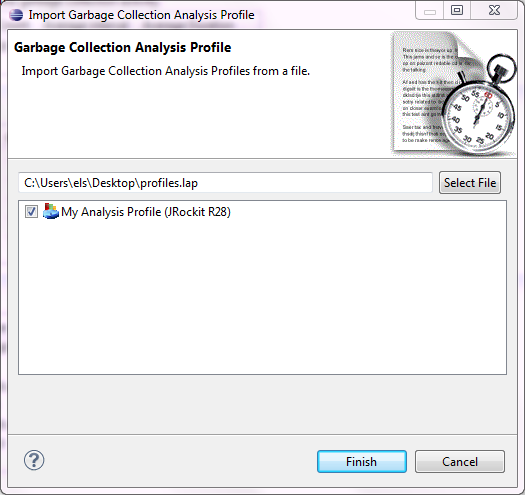
\includegraphics[width=10cm]{images/tutorial_importprofile}
        	\caption{Profil importieren}
\end{figure}

\section{Garbage Collection Analyse}
\subsection{Standardauswertung}
Sofern in der Ansicht \textit{Profile} kein Profil selektiert ist, wird mit Doppelklick auf eine importierte Logdatei die Standardauswertung geöffnet. Die Standardauswertung besteht aus drei unterschiedlichen Tabs. Der erste Tab zeigt eine Zusammenfassung der Garbage Collection, der zweite Tab den Verlauf des benötigten Speichers auf dem Heap über die Zeit, und der dritte Tab die Dauer der einzelnen Garbage Collection Zyklen über die Zeit. 

\subsubsection{Zusammenfassung}
 \begin{figure}[H]
  	\centering
    	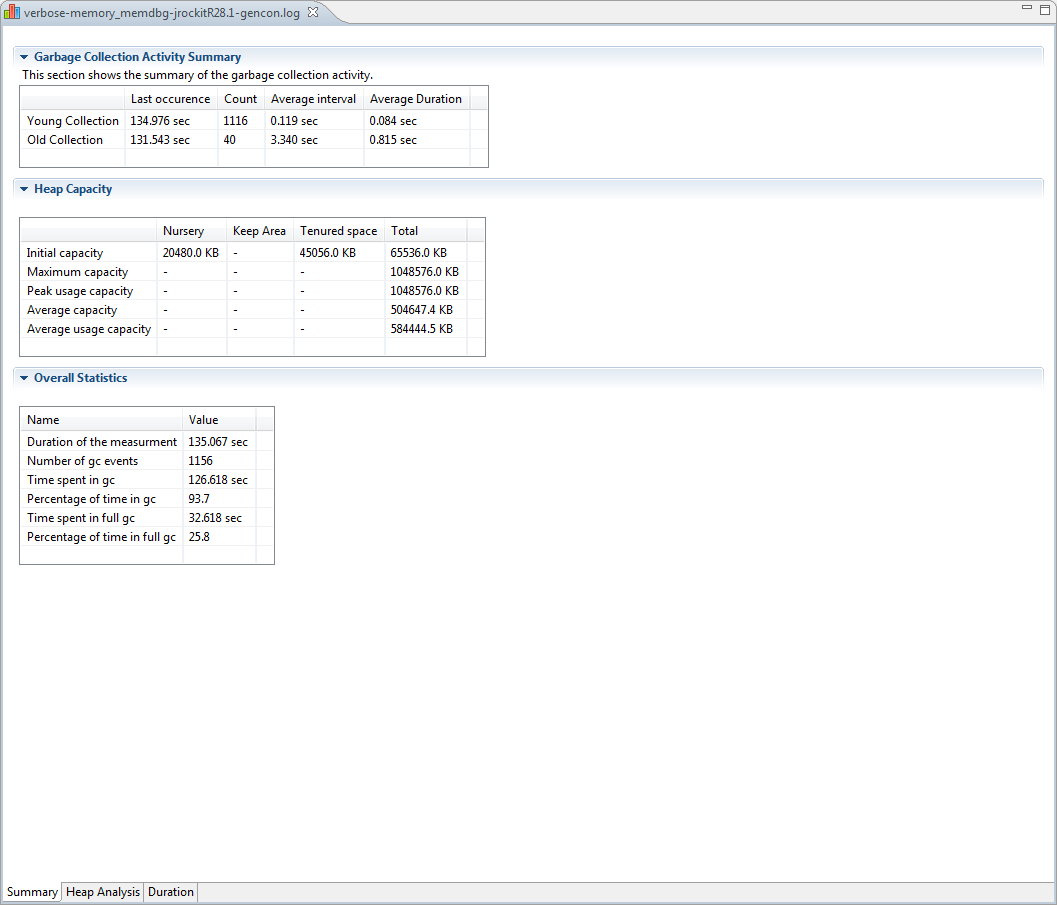
\includegraphics[width=15cm]{images/tutorial_standardreport_statistics}
        	\caption{Standardauswertung: Zusammenfassung}
\end{figure}

\subsubsection{Heap Analyse}
 \begin{figure}[H]
  	\centering
    	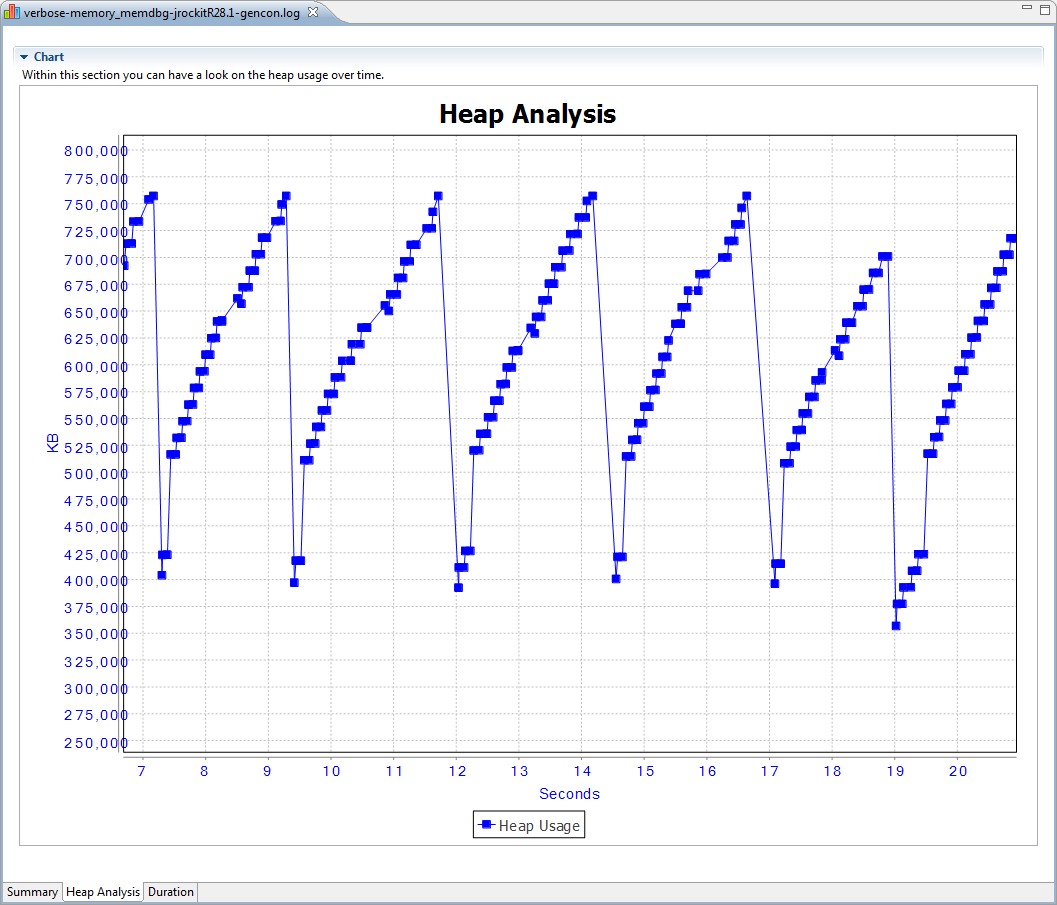
\includegraphics[width=15cm]{images/tutorial_standardreport_heapanalysis}
        	\caption{Standardauswertung: Heap Analyse}
\end{figure}

\subsubsection{Dauer Garbage Collection}
 \begin{figure}[H]
  	\centering
    	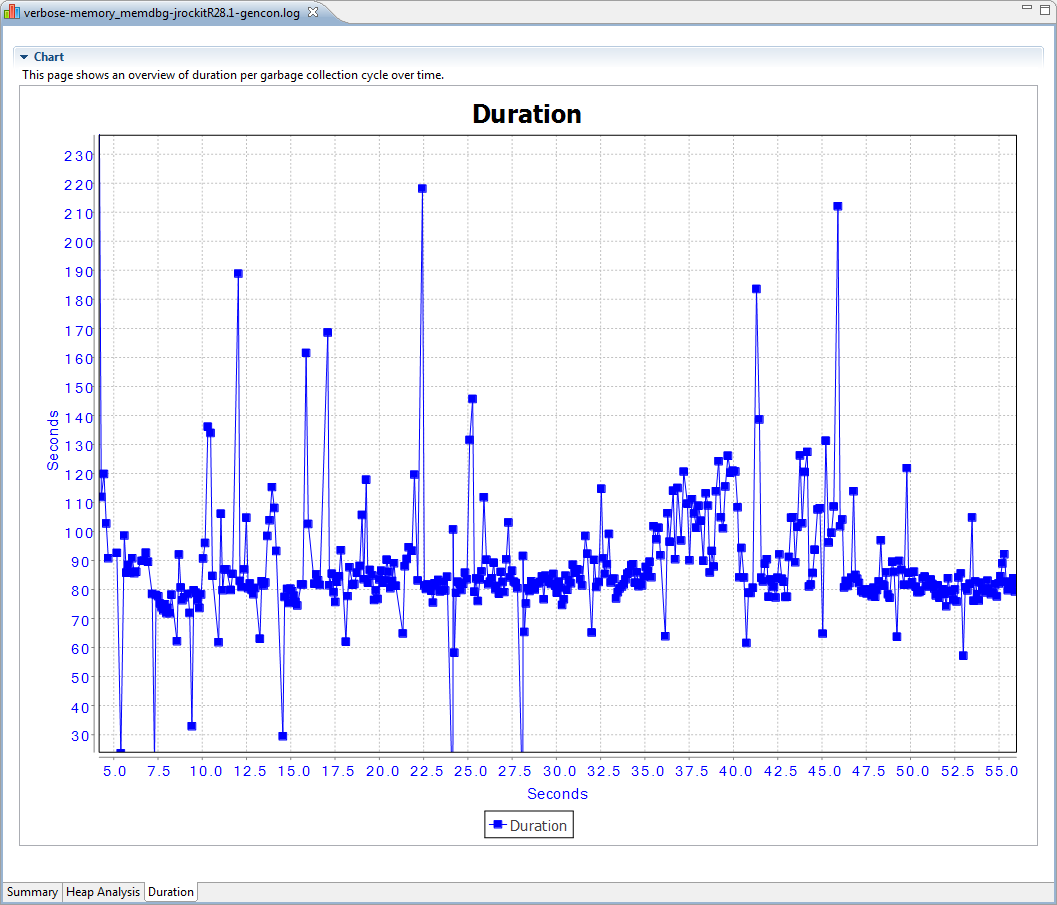
\includegraphics[width=15cm]{images/tutorial_standardreport_duration}
        	\caption{Standardauswertung: Dauer Garbage Collection}
\end{figure}



\subsection{Benutzerdefinierte Auswertung (Profile)}
Die benutzerdefinierte Auswertung wird geöffnet, indem man vor dem Öffnen einer Datei in der Ansicht \textit{Profile} ein Profil selektiert. 
 \begin{figure}[H]
  	\centering
    	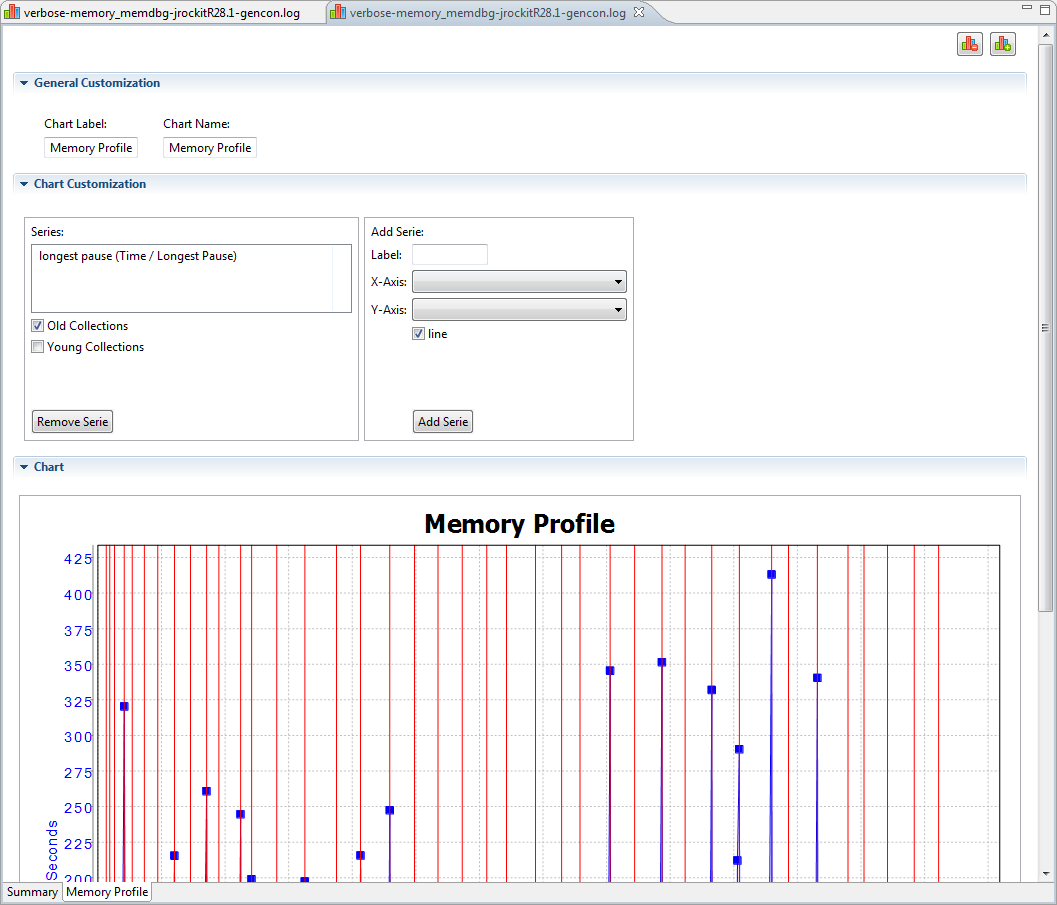
\includegraphics[width=15cm]{images/tutorial_custom_report}
        	\caption{Standardauswertung: Zusammenfassung}
\end{figure}
Im Abschnitt \textit{Generelle Anpassungen} können die Namen von Tab  und Diagramm definiert werden. Im Abschnitt \textit{Anpassung Diagramm} können neue Serien auf das Diagramm hinzugefügt werden. Dabei können pro Serie die Werte für X-, Y-Achse und ein paar Eigenschaften angegeben werden. Das jeweilige Ende einer Garbage Collection kann als vertikale Linien in rot (Old Collections) oder blau (Young Collections) angezeigt werden.

